% This is LLNCS.DEM the demonstration file of
% the LaTeX macro package from Springer-Verlag
% for Lecture Notes in Computer Science,
% version 2.4 for LaTeX2e as of 16. April 2010
%
\documentclass{llncs}
%
\usepackage[english]{babel}
\usepackage[utf8]{inputenc}
\usepackage{xspace}
\usepackage{url}
\usepackage{makeidx}  % allows for indexgeneration
\usepackage{graphicx}
\usepackage{float}
\usepackage{hyperref}
\usepackage{verbatim}
\usepackage{tikz}
\usetikzlibrary{shapes,arrows}



\newcommand{\constituency}[2]{\textit{#1} : \textit{#2}}
\newcommand{\obligation}[2]{\textit{#1} : \triangle \textit{#2}}
\newcommand{\uniqueness}[2]{\textit{#1} : \textit{#2}\,!}
\newcommand{\precedence}[3]{\textit{#1} : \textit{#2} \prec \textit{#3}}
\newcommand{\requirement}[3]{\textit{#1} : \textit{#2} \Rightarrow \textit{#3}}
\newcommand{\exclusion}[3]{\textit{#1} : \textit{#2} \not\Leftrightarrow \textit{#3}}
\newcommand{\dependency}[3]{\textit{#1} : \textit{#2} \sim \textit{#3}}

\newcommand{\PN}{\textit{PN}\xspace}
\newcommand{\NP}{\textit{NP}\xspace}
\newcommand{\VP}{\textit{VP}\xspace}
\newcommand{\Se}{\textit{S}\xspace}
\newcommand{\N}{\textit{N}\xspace}
\newcommand{\V}{\textit{V}\xspace}
\newcommand{\D}{\textit{D}\xspace}
\newcommand{\ADJ}{\textit{ADJ}\xspace}

%
\begin{document}
%
\bibliographystyle{splncs03}% the recommended bibstyle
%
\mainmatter              % start of the contributions
%
\title{On Failure-Driven Constraint-Based Parsing through CHRG\thanks{This paper was supported by NSERC  Discovery grant 31611024, and developed during a visit to Universidade Nova de Lisboa}}
%
\titlerunning{On Failure-Driven Parsing}  % abbreviated title (for running head)
%                                     also used for the TOC unless
%                                     \toctitle is used
%
\author{Veronica Dahl\inst{1}, Sinan Eğilmez\inst{2}, João Martins\inst{2,3} and J. Emilio Miralles\inst{1}}
%
\authorrunning{V.~Dahl, S.~Egilmez, J.~Martins, J.~E.~Miralles} % abbreviated author list (for running head)
%
%%%% list of authors for the TOC (use if author list has to be modified)
\tocauthor{V.~Dahl, S.~Egilmez, J.~Martins, J.~E.~Miralles}
%
\institute{Simon Fraser University, Burnaby, BC V5A-1S6, Canada,\\
\email{veronica@cs.sfu.ca, emiralle@sfu.ca}
\and
CENTRIA and Departamento de Informática, FCT, Universidade Nova de Lisboa
\and
Computer Science Department, Carnegie Mellon University, Pittsburgh PA\\
\email{s.egilmez@campus.fct.unl.pt, jmartins@cs.cmu.edu}}
\maketitle              % typeset the title of the contribution


\begin{abstract}

In this article we adapt and further develop  a CHRG parsing technique which was initially conceived in the context of grammar induction for Womb Grammars \cite{DM12}. We also show that applying it to constraint-based linguistic formalisms such as Property Grammars \cite{Blache} can yield truly direct implementations of specialized parsers that focus on ungrammaticality detection and correction.

\end{abstract}
%

\section{Introduction}
% 

Since the advent of CHR \cite{Fruhwirth98} and of its grammatical counterpart CHRG \cite{Christiansen01}, constraint-based linguistic formalisms can materialize through fairly direct meth\-odologies.   In this article we study several advantages of doing so. Efficiency-wise, direct CHRG renditions of linguistic constraints promote efficiency by their very adherence to  the constraint solving framework. We propose to enhance them further through exploiting our novel  methodology, arrived at through our work on grammar induction \cite{DM12}, of  checking only for falsification of most constraints in PG \cite{Blache} and similar formalisms.
%  

Constraint-based theories of grammar  are by now widespread in computational linguistics, but there is still no general consensus on what comes under that umbrella. 

Shieber's initial characterization of constraint-based theories in terms of common threads such as modularity, declarative constructs and partial information  \cite{Shieber} has been influential to this day, partly because it is wide enough to accommodate a variety of grammar theories springing from different fields -- linguistics, computational linguistics and artificial intelligence. However such threads  are present in many formalisms that would not be viewed as constraint based in the computational science of constraint solving  as  originally described \cite{Waltz}.

The constraint solving paradigm of computing sciences has proved very successful in greatly reducing search spaces by stating a problem in terms of constraints on domain-associated variables, whose possible values are automatically and successively narrowed down through constraint solving into values that represent a solution, if one exists. It would be therefore most interesting from the point of view of efficiency to consider to what extent the so-called constraint based grammar models fit into the constraint solving model strictly speaking.

The candidate constraint-based theories of grammar to consider, if we follow Shieber's characterization,   range widely from augmented transition networks \cite{Woods1970} to logic grammars \cite{AD89}, to  recent and highly specialized formalisms such as \cite{Muresan2010}, or Womb grammar parsing \cite{DM12}.
Among them, the Property Grammar (PG) framework \cite{Blache} stands out as an effort to completely describe a grammar in terms of constraints. It  defines phrase acceptability in terms of the properties or constraints that must be satisfied by groups of categories (e.g. English noun phrases can be described through a few constraints such as precedence (a determiner must precede a noun), uniqueness (there must be only one determiner), exclusion (an adjective phrase must not coexist with a superlative), and so on). Rather than resulting in either a parse tree or failure, such frameworks characterize a sentence through the list of the constraints a phrase satisfies and the list of constraints it violates, so that even incorrect or incomplete phrases will be parsed to the extent that they can, rather than simply failing.

Because of their sole reliance of constraints, Property Grammars are a main candidate for direct implementation in terms of constraint solving. However the only works which incorporate direct implementation to some extent are \cite{BM00}, \cite{DB04}, \cite{logcom13DuchierEtAl} and Womb Parsing \cite{DM12}.  Of these, the only one that does not need to  calculate all constraints between every pair of constituents is \cite{DM12}. Instead, it checks  constraints  only for failure. This works well in the context of  grammar induction. In the present paper we examine how to adapt that work to  parsing sentences rather than inducing grammars, while retaining both the search space reduction obtained by the failure-driven focus  and the direct implementation character  (in the constraint-solving sense)  of \cite{DM12}. 

\section{Background}

\subsection{Property Grammars}

The idea of representing a language's grammar solely through properties between constituents was first proposed as a theoretical formalism by Gabriel Bes \cite{Bes}, and reworked by Philippe Blache into Property Grammars  \cite{Blache,BB01}. Computationally, it relates to Gazdar and Pullum's dissociation of phrase structure rules into the two properties of Immediate Dominance (called constituency in the PG literature) and Linear Precedence (called either precedence or linearity in PG) \cite{IDLP}.   It presently comprises the following seven categories (we adopt the handy notation of  \cite{logcom13DuchierEtAl} for readability, and the same example):

\begin{description}
  \item[Constituency] $\constituency{A}{S}$, children must have categories in the set $S$
  \item[Obligation] $\obligation{A}{B}$, at least one $B$ child
  \item[Uniqueness] $\uniqueness{A}{B}$, at most one $B$ child
  \item[Precedence] $\precedence{A}{B}{C}$, $B$ children precede $C$ children
  \item[Requirement]$\requirement{A}{B}{C}$, if $B$ is a child, then also $C$ is a child
  \item[Exclusion]$\exclusion{A}{B}{C}$, $B$ and $C$ children are mutually exclusive
  \item[Dependency]$\dependency{A}{B}{C}$, the features of C1 and C2 are the same
\end{description}

This paper will handle full sentences, so that we will generally denote determiners by \D, nouns by \N, personal nouns by \PN, verbs by \V, noun phrases by \NP, verb phrases by \VP and sentences by \Se.

\begin{example} For example, the context free rules $\NP\to D\ N$ and $\NP \to N$, which determine what a noun phrase is, can be translated into the following equivalent constraints: $\constituency{NP}{\{D, N\}}, \uniqueness{NP}{D}, \obligation{NP}{N}, \uniqueness{NP}{N}, \precedence{NP}{D}{N}, \constituency{D}{\{\}}, \constituency{N}{\{\}}$.
\end{example}

The larger number of constraints allows us to perceive and understand the grammar rules in a more detailed fashion. Furthermore, this finer granularity can be exploited: in some of the literature on PG there is the possibility of declaring some constraints as relaxable. The failure of relaxable contraints is signalled in the output, but does not block the entire sentence's analysis.  Implementations not including constraint relaxation capabilities implicitly consider all properties as relaxable.


 
%
\subsection{Womb Grammar Parsing}

%
 Womb Grammar Parsing   is a constraint-based parsing methodology developed in 2012 \cite {DM12}, motivated by the need to aid the world's linguist uncover the syntax of the many languages that are not being studied for lack of resources.
It was designed to induce a target language's syntax from the known syntax of a source language plus a representative corpus of correct sentences in the target language and the target language's known lexicon.  It was presented in two versions: Hybrid Womb Parsing, in which the source language is an existing language for which the syntax is known, and Universal Womb Parsing,  in which the source syntax is a hypothetical universal grammar of the authors' own devise, which contains all possible properties between pairs of constituents.

Womb Parsing has the originality of addressing through constraint solving a problem  which more usually is cast as a machine learning problem. Additionally, it fully applies the technique of using  linguistic information from one language for the task of describing another language, which until then had  yielded good results only for specific tasks---such as disambiguating the other language \cite{BurkKlein:2008}, or fixing morphological or syntactic differences by modifying tree-based rules \cite{Nicolas:towardsefficient}---rather than for syntax induction.



%

\section{From Womb Parsing to Direct PG Parsing}

\begin{comment}
The way Womb Parsing works is by adjusting the  constraints given in the source grammar so that they suit the input corpus being parsed. Since this corpus is chosen to be correct and representative, we're justified for instance in deleting any constraints that the corpus violates.

As an example, if the source grammar contains the precedence constraint $\precedence{np}{n}{adj}$, encoded as:

\begin{verbatim}
(1) g(precedence(np, n, adj)).  
\end{verbatim}

and there is an input noun phrase in which an adjective precedes a noun, the following CHRG rule will apply and delete the above precedence constraint (via the call to "update"):

\begin{verbatim}
(2) !word(C2,Phrase_,_), ... , !word(C1,Phrase,_,_), 
    g(precedence(Phrase, C1, C2))}
    <:> {update(precedence(Phrase,C1,C2,Phrase)}
\end{verbatim}
Each word is stored in a CHRG symbol word/3, along with its category, its mother constituent,  and traits (i.e. word(n,np,[sing,masc],livre)). Since the CHRG parse predicate stores and abstracts the position of each word in the sentence, this simpagation rule is triggered when a word of category C2 comes before one of category C1, given the existence of the grammar constraint that C1 must precede C2 within a phrase of type Phrase. In CHRG syntax the symbols prefixed with exclamation points are kept, while the ones without are replaced by the body of the rule.  Each of the properties dealt with has similar rules associated with it.

\end{comment}
\subsection{The Main Idea}

Womb Parsing works  by adjusting the  constraints given in the source grammar until they suit the input corpus. Since this corpus is chosen to be correct and representative, we're justified e.g. in deleting any constraints that the corpus violates.

For instance, if the source grammar contains the precedence constraint $\precedence{\NP}{\N}{\ADJ}$
and there is an input noun phrase in which an adjective precedes a noun, a CHRG rule will apply and delete the above precedence constraint. Thus, the constraint was checked for violation, not satisfaction.

Each of the properties in PG has similar CHRG rules associated with it. Our proposal here is to adapt these rules into admitting constraint relaxation and signalling failure of non-relaxed constraints that do not satisfy input sentences, rather than adjusting the constraints that failed. Furthermore, the method works on complex sentences rather than just noun phrases.

\subsection{Significance}

The Womb Parsing method of adapting another language's grammar constraints  until they suit the target language's representative input corpus can inspire a new way of viewing the PG \emph{parsing problem}, in which  constraints are tested only for failure. In contrast, all previous methods exhaustively test each constraint for all constituents that can participate in it. Concretely, a notion  not unlike obligation can be used to identify new phrases, and those phrases can be tentatively expanded from nearby constituents.

\begin{example}In ``john eats an apple'', the noun indicates the existence of a noun phrase. Because noun $\constituency{NP}{\{D, N\}}$, then the tentative noun phrase starting at ``apple'' can include ``an'' but not ``eats'', since it can only be constituted by determiners and nouns. This is the constraint-satisfaction criterion for expansion.
\end{example}

For each tentatively expanded phrase, all other constraints are tested for \emph{failure} only. The phrase is allowed to expand only if either no constraint fails, or all constraints that fail have been declared as relaxable. Exhaustive satisfaction check is thus replaced by a smart guided search for a falsifying assignment. This is appropriate provided that  the set of satisfied constraints is the exact complement of the set of failed constraints - an assumption that seems reasonable, and that we make. In this case, it follows that we do not need to check the satisfied constraints.  Just as for grammar induction we do not need to touch the constraints of the source grammar that do work for the target grammar,  we can for PGs  only actively check  the constraints that do not hold. Should we need to explicitly output those that hold, they could be inferred  from the list of constraints that must be satisfied plus those output as unsatisfied, at less computational cost than the usual practice of evaluating  all constraints between every pair of constituents, or of adding heuristics to reduce the search space.

This is significant because deep parsing with Property Grammars is theoretically exponential in the number of categories of the grammar and the size of the sentence to parse \cite{vanRullen2005}. Since all previous approaches to PG parsing (except for Womb Parsing) have to calculate all constraints between every pair of constituents, and since the number of failed constraints will in general be much smaller than the number of satisfied constraints,  any parsing methodology that manages to mostly check the failed ones will have a substantial efficiency advantage. If moreover the failed constraints can be checked in the automatic workings of a truly constraint solving formulation like our CHRG one, by means of letting those rules that apply to each particular input sentence trigger, we now have more realistic hopes of turning (our version of) the PG paradigm, which we  call Direct PG, into a useful, directly executable constraint-based theory of language. In this first paper we address this hope from the point of view of direct parsing for ungrammaticality detection.


\subsection{Phrase Determination}

In \cite {DM12}, where we only dealt with noun phrases, constituency did not need to be checked explicitly, because it followed from a lexicon made only from noun phrase constituents. The core idea was to start the noun phrase from its head noun, and try to expand it. Expansion would fail if any of the grammatical constraints failed.

More concretely, one expands instantiated categories, which are CHRG predicates of the type \texttt{iCat(Start, End, CategoryType, Attributes, Tree)}. Instantiated categories simply keep track of the location, attributes (gender and plurality) and parse tree of all categories, or phrase types, in a specific sentence (e.g. \N, \NP, etc).

\begin{example}[Instantiated categories] \label{ex:icat} Take the noun phrase ``an apple'' in French, or ``une pomme'', which is feminine. Parsing it results in the following instantiated categories.
\begin{verbatim}
            iCat(0, 1, det, [sing,fem], det(un))
            iCat(1, 2, n,   [sing,fem], n(pomme))
            iCat(0, 2, np,  [sing,fem],
              np(
                iCat(0, 1, det, [sing,fem], det(un)),
                iCat(1, 2, n,   [sing,fem], n(pomme))
              )
            )
\end{verbatim}

Notice that the \NP inherits the attributes of the underlying \N, thus implementing their dependency constraints; and that a tree is built as a side-effect from parsing.\end{example}

Since in this work we need to treat whole sentences rather than just noun phrases, some additional considerations are necessary:
\begin{itemize}
  \item Whereas in \cite {DM12} it was implicit that noun phrases grew from their head nouns, for full sentences each phrasal category must explicitly have its own \emph{head}. These heads follow closely from the grammar itself and the obligation constraints it implies. In our case, we have:
\begin{verbatim}  head(n, np). head(pn, np). head(v, vp). head(vp, sentence).\end{verbatim}
  
  \item For full sentences, the extra complexity requires phrases to be treated in a specific ordering. For example, because a verb phrase can contain noun phrases, noun phrases should be parsed before verb phrases, and verb phrases should be parsed before sentences. The ordering is currently specified as part of the grammar, though it could be induced from the directed constituency graph implied by a grammar. For the sentences we consider, the following order is used:
\begin{verbatim}                  parseOrder([np,vp,sentence]).\end{verbatim}

After all categories of the type at the head of the list have been parsed and expanded, the algorithm moves on to the next category.
\begin{verbatim}               parseOrder([_|L]) <=> parseOrder(L).
\end{verbatim}
  
  \item While the PG formalism per se does not care about syntactic trees (it just characterizes an input sentence through its lists of satisfied and unsatisfied properties), they are important for complex sentences, and are thus built as a side-effect of the algorithm. Not only is this handy to the traditional way in which linguists are used to thinking of a parse result, but it is also useful to ensure that the constraints apply on immediate daughters only. For instance, consider the parse tree of ``john eats an apple'' in Figure \ref{fig:tree}. It contains two noun phrases, ``john'' and ``an apple'', but only `john'' is a direct daughter of the sentence (``an apple'' is a direct daughter of the verb phrase ``eats an apple''). Therefore, the uniqueness of a noun phrase $\NP$ in a sentence \Se, $\uniqueness{\Se}{\NP}$, should not fail.

\begin{figure}[H]
\begin{center}
  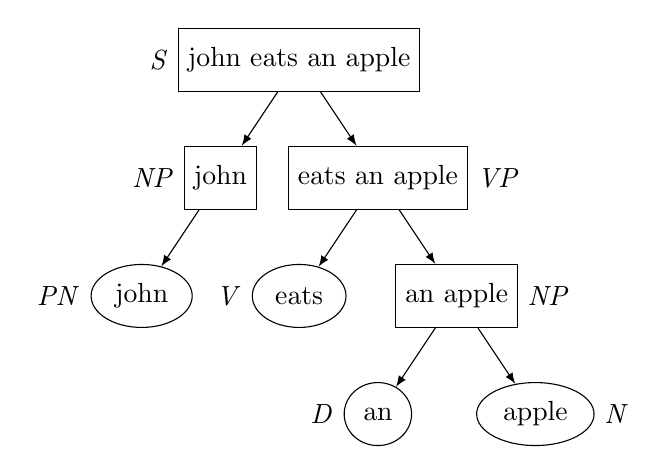
\begin{tikzpicture}[>=latex, auto] 
  \tikzstyle{argument}=[draw, shape=rectangle, minimum size=8mm];
  \tikzstyle{leaf}=[draw, shape=ellipse, minimum size=8mm];
  \node [argument, label=left:\Se] (S) at (1,0){john eats an apple};
  \node [argument, label=left:\NP] (NPP) at (0,-1.5){john};
  \node [leaf, label=left:\PN] (PN) at (-1,-3){john};
  \node [argument, label=right:\VP] (VP) at (2, -1.5){eats an apple};
  \node [leaf, label=left:\V] (V) at (1, -3){eats};
  \node [argument, label=right:\NP] (NP) at (3, -3){an apple};
  \node [leaf, label=left:\D] (D) at (2, -4.5){an};
  \node [leaf, label=right:\N] (N) at (4, -4.5){apple};
  \draw [->] (S) to (NPP);
  \draw [->] (S) to (VP);
  \draw [->] (NPP) to (PN);
  \draw [->] (VP) to (V);
  \draw [->] (VP) to (NP);
  \draw [->] (NP) to (D);
  \draw [->] (NP) to (N);
  %\node [argument, label=left:$\alpha_1/\beta_1$](a) at (0, 0){$\cdot$};
  %\node [labelling](pclabel) at (0,4.25){\textbf{Power Controller}};
  %\node [argument, label=above:\text{Normal(5, 1)}](pc) at (0, 3){$\cdot$};
  %\draw [<-] (pc) to [loop left] (pc) node [midway, text width=1.9cm]{$\asnd[g_{o}][G_o]$ p = 0.4}; % Transmitting
  \end{tikzpicture}
  \caption{Parse tree of the sentence.}
  \label{fig:tree}
  \end{center}
\end{figure}
\end{itemize}

Taking all these considerations into account, the rules for creating new categories from their heads is the following.
\begin{verbatim}
iCat(Comp,Attr,Tree):(N1,N2), {parseOrder([Cat|_])}
  ::> head(Comp, Cat), NewTree=..[Cat,iCat(N1,N2,Comp,Attr,Tree)]
  | iCat(Cat, Attr, NewTree).
\end{verbatim}

This rule is found after the expansion and constraint satisfaction checks. This means it will only apply if \texttt{iCat(Comp,Attr,Tree):(N1,N2)} has been maximally expanded so that it does not violate unrelaxable constraints. After this rule applies, there will be a new instantiated category, which will in turn be expanded maximally, and checked against the constraints. Once no more checks or expansions can be done on any category of the current type, the parsing moves on to the next category type given by \texttt{parseOrder\textbackslash 1}.

The expansion rules are a little more verbose, but the reader should now be acquainted with most predicates used. We present here a simplified version of the left-expansion rule (the right-expansion rule is symmetric).

\begin{verbatim}
  !iCat(Comp, Attr1, Tree1):(N1,N2), 
  iCat(Cat, Attr2, Tree2):(N2,N3),
  !{tpl(constituency(Cat, L))},!{evil(EL)},
  !{parseOrder([Cat|_])}
 <:> member(Comp, L),
     buildTree(Cat, iCat(N1,N2,Comp, Attr1, Tree1),
                    iCat(N2,N3,Cat , Attr2, Tree2),
                    Tree)
 | iCat(Cat, Attr2, Tree):(N1,N3).
\end{verbatim}

Expansion considers two adjacent categories only. The component category will remain (e.g. the \D of an \NP), whereas the \texttt{iCat} of the expanding category is replaced by its expanded version. This rule is guided by constituency, so that senseless expansions do not occur, e.g. \NP can be expanded to include an adjacent \D (to the left or right!) but not a \V. A discussion of the location of the expansion rules is more appropriately found in Section \ref{ssec:constrs}.

Notice that only constituency is checked at this point. The other constraints are deferred until after the expansion. Whenever an expansion causes some constraint to be falsified, a rule will fire to alert us to that effect. If the falsified constraint is relaxable, the algorithm is allowed to continue. If it is not, however, the expansion that caused the falsification is retracted, and reverts back to its unexpanded predecessor.

We now present a couple of examples of such constraint violation rules for the reader's benefit. First, the precedence rule $\precedence{Cat}{C1}{C2}$:

\begin{verbatim}
  iCat(C2,Attr2,Tree2):(N1,N2), ... , % Found C2
  iCat(C1,Attr1,Tree1):(N3,N4),       % Found C1 (after C2)
  {iCat(N5,N6,Cat,_,Tree)},           % Found Cat (somewhere)
  {tpl(precedence(Cat,C1,C2))}        % Cat: C1 < C2
  ::> % Cat encompasses C1 and C2
      N5 =< N1, N4 =< N6, Tree=..[Cat|T],
      % C1 and C2 are direct daughters of Cat
      member(iCat(N1,N2,C2,Attr2,Tree2), T),
      member(iCat(N3,N4,C1,Attr1,Tree1), T)
  | falsify(precedence(Cat,C1,C2)):(N1,N4),   % Precedence falsified!
    {failed(g(N1,N4,precedence(Cat,C1,C2)))}. % Failure of tentative category
\end{verbatim}

\subsection{Algorithm overview}

Since the specifics of the algorithm can get a little involved, it is perhaps helpful to abstract away the rules, their positions and the order in which they fire. In fact, the algorithm is conceptually extremely simple.

\begin{enumerate}
\item If there is an instantiated category of the type being handled (e.g. \NP, \VP, \Se) that can be expanded without violating unrelaxable constraints, the expansion is carried out. Violated relaxable constraints are stored for reference.
\item If no more expansions are possible and there is an instantiated category can be a head for the category being handled, then a new instantiated category of that type is created from the head.
\item If no more expansions are possible and there are no more potential heads, the algorithm proceeds to handle the next category type.
\end{enumerate}

\begin{example}
  Consider our running example of ``john eats an apple'' again and the following context free grammar (stated in bottom-up fashion), $\PN \to \NP$; $D, N \to \NP$; $V,\NP \to \VP$; $NP, \VP \to S$, where $\PN$ is a proper noun and $S$ a sentence. \N and \PN are the heads of \NP, \V of \VP and \VP of \Se.
  
  The parse ordering associated with these rules is $\NP,\VP,\Se$. We will consider the constraints induced from the grammar rather than the grammar itself.

The algorithm thus starts by creating the leaf instantiated categories for the \PN, \N, \D, and \V words. Then, the \NP{}s ``john'' and ``apple'' are created from the respective \PN and \N heads. The \NP ``apple'' is expandable to ``an apple'', and then no more expansions are possible for ``john'' or ``an appple', since $\constituency{NP}{\{D, N\}}$.

The algorithm thus moves to \VP{}s, and create one from the \V head ``eats''. Since $\constituency{VP}{\{V, NP\}}$, the \VP is expandable to both left, for ``john'' and right, for ``an apple''. The right expansion succeeds without problems. The left expansion falsifies the precedence $\precedence{VP}{V}{NP}$, and is therefore not carried out.

Since no more expansions are possible for \VP{}s, a \Se is created from the \VP and expanded to ``john'', creating he full sentence. However, suppose that $\precedence{VP}{V}{NP}$ were relaxable. Then, the \VP would expand both left and right, encompassing the whole sentence. With no more expansions possible, a sentence $S$ would be created from the \VP containing the whole sentence, thereby violating the obligation $\obligation{\Se}{\NP}$ (since the constraint requires \NP as a direct \emph{direct} daughter), and would thus be retracted. This parse would not result in a sentence. If that restriction were, in turn, relaxable, the parse would keep the \Se instead of retracting it.

If no constraints were relaxable, ``john eats apple'' would not parse a sentence \Se (or a \VP or even an \NP) because nouns must have determiners, i.e. $\requirement{NP}{N}{D}$. If that were relaxed, however, the entire sentence would be parsed with no further complications! This highlights the flexibility of the approach.
\end{example}

\subsection{Types of constraints, and their procedural implications}
\label{ssec:constrs}

As we have seen, our parsing algorithm's reliance on expansion from phrasal heads into allowable constituents for that phrase places  the constraints of constituency and head obligation in the category of non-relaxable, with all other constraints being relaxable.

For relaxable constraints we can identify a further, useful distinction: that between permanent and changeable constraints. Notice that CHRG rules  for constraints such as precedence can be allowed to apply  immediately after the two constituents they involve show up in the constraint store, no matter what stage of parsing we are at.  This is because as soon as the constraint can be evaluated, its value is \emph{permanent}. Once it fails, adding new constituents to the category cannot make it succeed, since e.g. two unordered elements will remain unordered even when adding more elements around them.  Accordingly, our methodology only checks for failure of permanent constraints, regardless of at what stage they fail.

Other constraints, which we call \emph{changing} constraints, can change in their  evaluation by the incorporation of one
more category into a given phrase for which, without this added category, the
constraint had an opposite value. Thus, for ``a red apple'',  at the point in which ``red'' and ``apple'' have been grouped into a noun phrase, this noun phrase will fail the constraint that a noun requires a determiner. However subsequent expansion of the noun phrase into ``a red apple'' will remedy the failure. This subtype of changing constraints is called \emph{recoverable}. For recoverable constraints, we simply wait until a phrase has been maximally expanded before testing whether they fail. We effect this by applying all expansion rules  before checking any recoverable constraints.

For the other type of changing constraints, called \emph{filtering} constraints, the addition of one more element into a phrase might make the constraint fail where it succeeded before. As an example, while unicity of determiner holds for ``the book'', it no longer holds for ``the the book''. Since the rules that check this type of constraint are triggered only when the constraint fails (e.g. when two determiners show up inside a noun phrase), there is no need for waiting mechanisms, or for any maximal expansion to precede their checking. In this sense our approach is much more focused than previous ones, as a consequence of better fitting the constraint-solving model. 

% TODO add rules here and explain order

\subsection{Constraint Relaxation}

Constraint relaxation is indicated by the user as part of the grammar's definition, through a special system predicate \texttt{relaxable(L)}. Any constraints inside the list \texttt{L} can be relaxed; the others cannot. If all the \emph{permanent} constraints that are falsified during a phrase's expansion are relaxable, the constraints are simply added to a list of relaxed constraints and the expansion is accepted.  \emph{Changing} constraints are handled slightly differently. As seen, these should only be evaluated once the phrase cannot be expanded anymore. If, at that stage, all falsified changing constraints are relaxable, then the phrase is accepted, and furthermore allowed to be considered as a head of a more complex phrase.


\section{Concluding Remarks}

We have presented a novel parsing methodology inspired from Womb Grammar Parsing which greatly reduced the combinatorial explosion inherent in PG parsing by three main contributions: a) a truly direct constraint-solving materialization of constraints,  b) a great reduction of the number of constraints to be evaluated, through expressing most constraints in terms of failure only, and c) relaxation handling, which is not always present  in previous  PG renditions.

While a formal comparative complexity analysis would require a previous underlying  analysis of the disparate implementation means of the various formulations, we can intuitively trust that our two main contributions above mentioned are bound to enable a much greater degree of efficiency than  was previously possible. Roughly speaking, \cite{DB04} encodes the input PG into a set of CHRG rules that directly interpret the grammar in terms of satisfied or relaxed constraints, which are then propagated while a syntactic tree is built as a side effect. For efficiency, the implementation controls  the way in which a constraint is selected for evaluation, but still, the failure or success value of all constraints among every pair of constituents is exhaustively calculated or propagated.  \cite{BM00} resorts to heuristics but remains highly combinatorially explosive, since it involves developing a complete table of satisfied and unsatisfied constraints for every pair of categories involved. \cite{logcom13DuchierEtAl} is even more combinatorially explosive but interestingly, develops a parsing architecture with  full reliance on constraint satisfaction, using classical constraint-based techniques such as branch-and-bound to select and propagate constraint evaluations. It also allows for the relaxation of constraints, by choosing those solutions that maximize the ratio between satisfied and unsatisfied properties - there is no control over which properties are relaxable, however. 

The approach in \cite{DB04}, like our own, also completes original assignments of categories with
new categories when they are inferred, and it exploits a similar distinction between permanent and changing constraints to minimize recalculation. However, they need to explicitly inherit permanent constraints at each step, and to recalculate and eventually update at each step the satisfaction value of changing constraints. In contrast, as we have seen, our parsing methodology allows us to  simply bypass the need to inherit the value of permanent constraints (through only checking them on maximal phrases), to postpone the checking of recoverable constraints until the phrase has been identified as maximal, and to only check for filtering constraints when and if they do fail. Also in this sense we obtain considerable efficiency gains.


 


%
% ---- Bibliography ----
%
\bibliography{CHR2013}

\newpage
\appendix
\section{Appendix: Code, examples}
For reviewing purposes, the code is available at the following repository: \url{http://www.cs.cmu.edu/~jmartins/ng.pl}. It was implemented using SWI-Prolog (\url{http://www.swi-prolog.org/}) and CHRG (\url{http://akira.ruc.dk/~henning/chrg/}).
The suggested way of running it is by installing SWI-Prolog, downloading our source code and the CHRG source and putting them in the same folder. Then, run SWI-Prolog using \texttt{swipl}, and at the prompt \texttt{?- compile(ng).}. To parse phrases, use, for instance, \texttt{?- doParse([jean, mange, une, pomme]).}
The output is hopefully self-evident, but the most important predicates are\\
\texttt{iCat(left\_bound, right\_bound, phrase\_type, attributes, syntax\_tree)},\\
which represents phrases, and of which you should feel free to ignore the last, very verbose argument, containing the syntax tree. Then, \texttt{evil/1} contains the list of retracted \texttt{iCat}s (due to constraint falsification), and the \texttt{unsat/1} contains the list of falsified but relaxed constraints.
\subsection{Grammar and suggested examples}
The grammar can be found in the \texttt{ng.pl} file, under the predicate \texttt{init\_grammar}, which initialises it. It contains a few suggested relaxable predicates, which should be run with the above example, \texttt{?- doParse([jean, mange, une, pomme]).}.
Another suggestion is running \texttt{?- doParse([jean, mange, pomme, une]).} \\ with no relaxable predicates, and running it with the suggested relaxation of \\ 
\texttt{precedence(np,det,n)}, also in the file. This will show that a failure at the very basic \NP level will not interfere with further parsing.
Other suggestions are \texttt{?- doParse([jean, mange, pomme]).}, by relaxing the requirement constraint between nouns and determiners, or \texttt{?- doParse([le, jean, mange, une, pomme]).} and the related exclusion constraint between \PN and \D.
It is also interesting to add or remove the constraint that \VP should have \NP (commented in the file), causing parsing to stop with \texttt{pomme, une} or just \texttt{pomme} with no determiner.


\end{document}
